\documentclass[tikz]{standalone}

\usepackage{mathtools}

\let\Im\relax
\DeclareMathOperator{\Im}{Im}
\let\Re\relax
\DeclareMathOperator{\Re}{Re}

\usetikzlibrary{decorations.pathmorphing}

\def\xr{5}
\def\yr{1}

\begin{document}
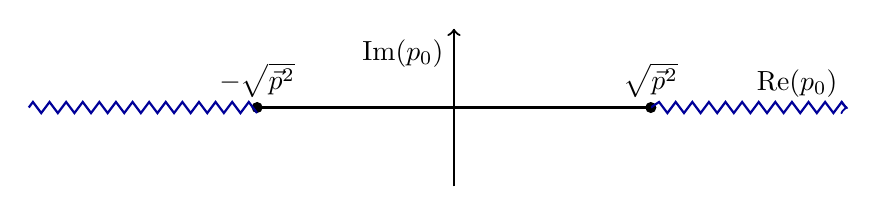
\begin{tikzpicture}[thick]

  % Labels
  \fill(-\xr/2, 0) circle (2pt) node[above] (l_branch) {$-\sqrt{\vec{p}^2}$} (\xr/2, 0) circle (2pt) node[above] (r_branch) {$\sqrt{\vec{p}^2}$};

  % Axes
  \draw[->, decorate, decoration={zigzag, segment length=6, amplitude=2}, blue!60!black] (-\xr-0.4, 0) -- (l_branch.south) (r_branch.south) -- (\xr, 0) node [above left, black] {$\Re(p_0)$};
  \draw(l_branch.south) -- (r_branch.south);
  \draw[->] (0, -\yr) -- (0, \yr) node[below left=0.1] {$\Im(p_0)$};

\end{tikzpicture}
\end{document}
